\chapter{Introduction}
\label{sec:intro}

Cuisenaire\textsuperscript{\textregistered} Rods \cite{TheCuise14:online} are an educational tool used in primary school mathematics classes to aid in the learning of, among other things, 'number bonds'. These are simple addition sums typically resulting in a round number like 10 or 20, such as $7+3=10$, which children learn as a foundation for more complex mathematical relationships. These are an important part of the Key Stage One (ages 5-7) curriculum in the UK, which is required to be followed by schools in England \cite{Mathemat26:online}. 

\begin{figure}[h] 
  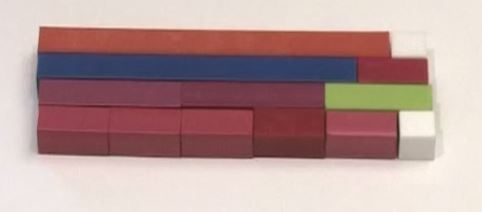
\includegraphics[width=0.75\textwidth]{rods.JPG}
  \centering
  \caption{A set of Cuisenaire\textsuperscript{\textregistered} Rods in use \cite{24Lesnom77:online}}
  \label{fig:rods}
\end{figure}

A set of rods consists of different-coloured cuboids, each colour of a different length, the smallest of which represents one unit. The rest of the rods are sized in multiples of this unit up to the longest rod, usually of size 10. Pupils are taught how different sized rods can be placed end-to-end in order to reach the target summation result, and are encouraged to find several alternate combinations of rods that add to the result, as demonstrated in Figure \ref{fig:rods}. This is a physical representation of number bonds, as the pupil can learn to associate a 7-rod (a rod of length 7) and a 3-rod forming a line of length 10 units with the mathematical concept that $7+3=10$. \\

The current disadvantage of the use of these rods is that in a class of dozens of students, it can be difficult for a teacher to monitor and track student progress. The teacher can survey the classroom, but is not capable of giving every student constant attention, so inevitably, poor progress sometimes goes unnoticed and students may fall behind without extra support. Additionally, students need to make a record of the work they have done, which can be difficult with the existing rods, as their use does not necessarily involve any written work.